\section{Discussion}\label{sec:discussion}

\begin{figure*}
    \centering
    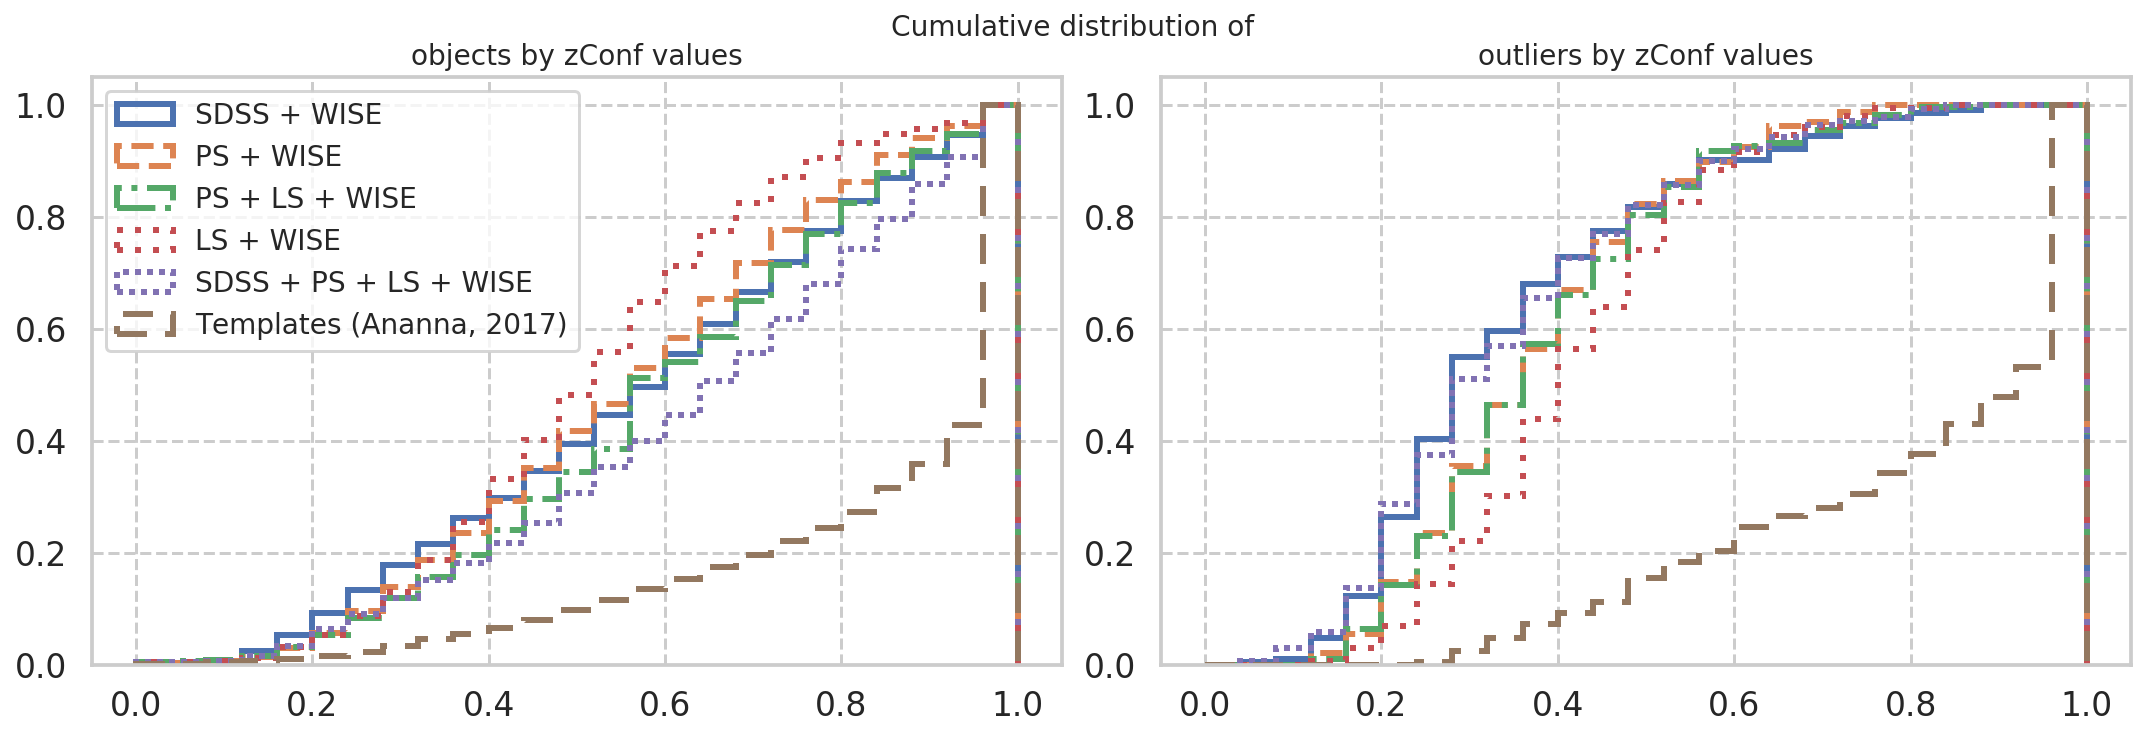
\includegraphics[width=\linewidth]{images/zconfs-s82x-a17.png}
    \caption{zConf cumulative distribution for entire Stripe82X dataset (left) and outliers (right)}
    \label{fig:zconfs-s82x-a17}
\end{figure*}

\begin{figure}
    \centering
    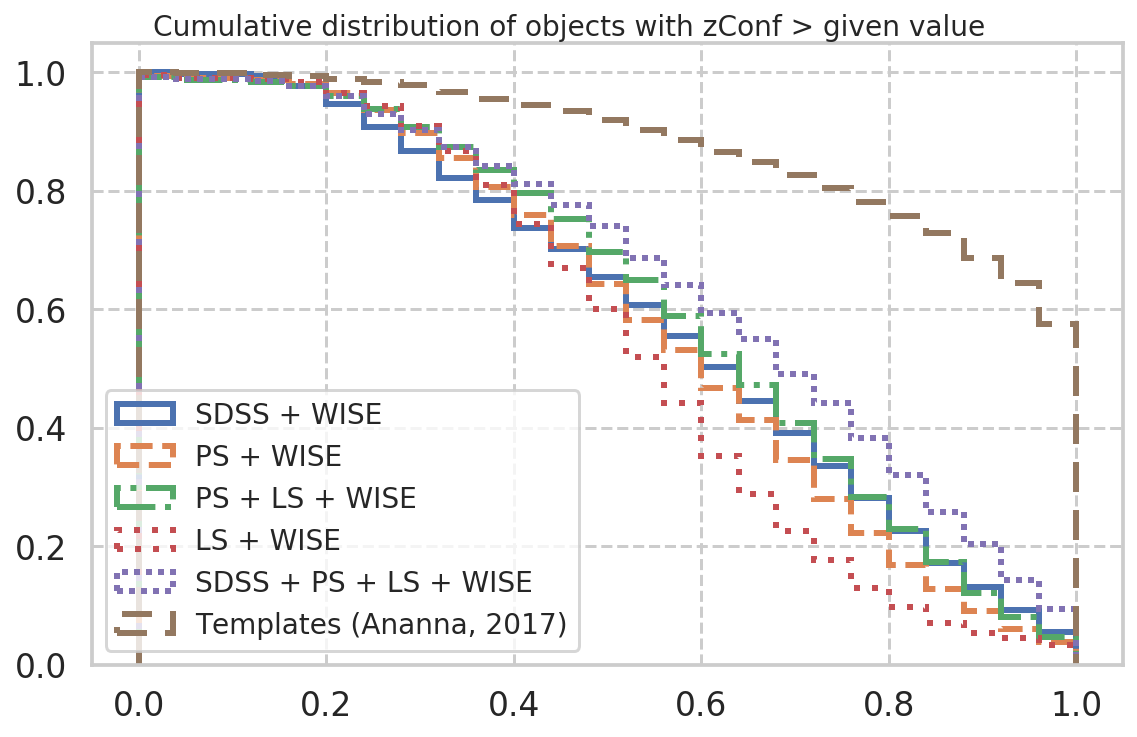
\includegraphics[width=\linewidth]{images/zconfs2-s82x-a17.png}
    \caption{zConf cumulative distribution for Stripe82X dataset}
    \label{fig:zconfs2-s82x-a17}
\end{figure}

Сказать, что результаты Brescia получены на кросс-валидации, у нас - нормальная обучающая выборка.

Обсудить покрытие неба моделями, что хотим хорошую точность на PanStarrs.
